\chapter*{Appendices}
\addcontentsline{toc}{chapter}{Appendices}

\appendix

\chapter{Rotation curves}\label{app:rotcurves}
A rotation curve shows the circular velocity as a function of
radius. We discuss here three different types of rotation curves, and
show examples of them in Figure~\ref{rotcurve}.

\section{Solid-body rotation} 
Think of a solid turntable, or a rotating DVD-disc. It rotates with a
constant angular speed $\Omega = \frac{V}{R} = {\rm constant}$. 
The circular velocity is therefore proportional to the radius: 
\begin{equation}
V \propto R. 
\end{equation}

\section{Keplerian rotation: the Solar system} 
\label{sect:kepler}
\begin{figure}[htbp]
\begin{center}
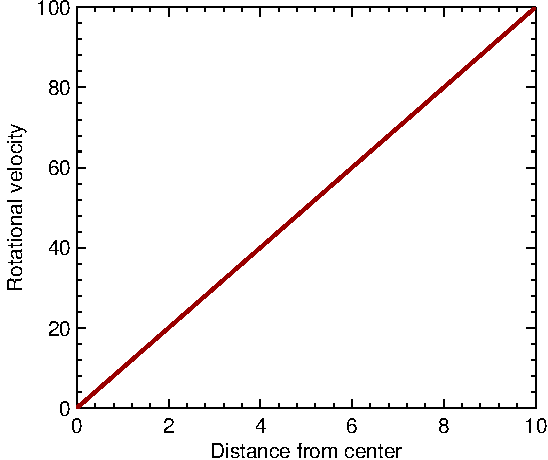
\includegraphics[width=8.2cm]{../figures/cdrot.pdf}
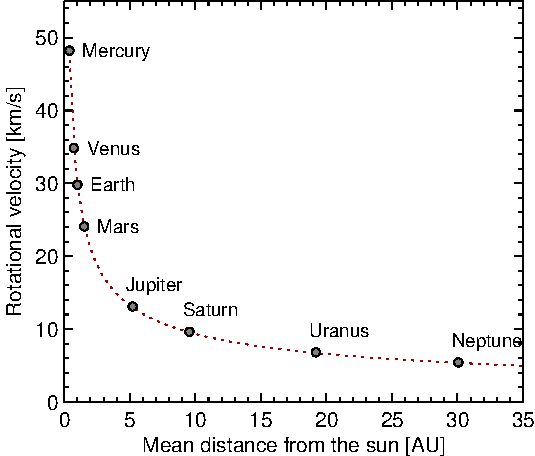
\includegraphics[width=8.2cm]{../figures/solsystrot.pdf}
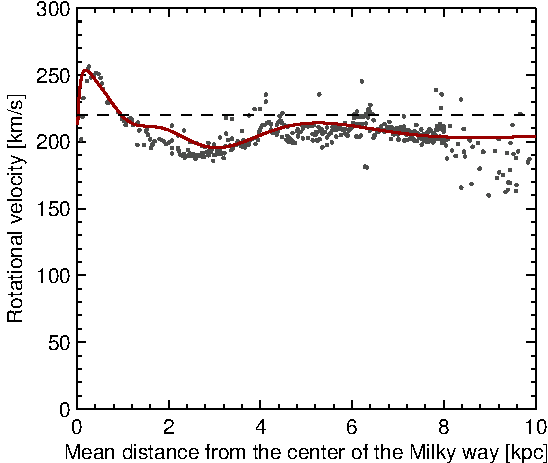
\includegraphics[width=8.2cm]{../figures/mwrot.pdf}
\end{center}
\caption{\emph{Top left}: solid body rotation (e.g. a rotating cd
  disc). \emph{Top right}: Rotational velocities of the planets of the
  Solar system. The line corresponds to Kepler's law
  (eq.~(\ref{kepler})) to which the planets show excellent agreement.
  The distance scale shown is in so-called \emph{Astronomical Units}
  (AU) which is the distance between the Earth and the Sun. $1
  \text{AU}=150\cdot 10^6 \text{km}$. \emph{Bottom}: the actual
  rotation curve of the Milky Way (dots) and a model describing it
  (solid line). Because there mass in the Milky Way is distributed
  across the galaxy, the rotation curve does not follow the Keplarian
  case, as it would if all the mass was to be in the center.(Data from Sofue et al, 2009) }
\label{rotcurve}
\end{figure}  

In the Solar system, the planets have a negligible mass compared to
the mass of the Sun. Therefore the center of mass of the Solar system
is very close to the center of the Sun. The centrifugal acceleration
from the planet's circular velocities counterbalances the
gravitational acceleration:
\begin{equation}
\frac{V^2}{R}= \frac{GM}{R^2}
\end{equation}
where $M$ is the mass and $G$ the gravitational constant.  The
rotation curve is said to be {\em Keplerian}, and the velocities
decrease with increasing radius:
\begin{equation}
\boxed{V_{\rm Keplerian}(R) = \sqrt{\frac{GM}{R}}.}
\label{kepler}
\end{equation}

\section{The rotation curve of a spiral galaxy}

Similarly, the rotation curve of a galaxy $V(R)$ shows the circular
velocity as a function of galacto-centric radius.  In contrast to the
rotation curve of systems like the Solar system with a large central
mass, most galaxies exhibit flat rotation curves, that is, $V(R)$
doesn't depend on $R$ beyond a certain radius:

\begin{equation}
\boxed{V_{\rm Galaxy}(R) \sim {\rm constant}}
\end{equation}

The angular velocity varies as $\Omega \propto 1/R$. Matter near the
center rotates with a larger angular speed than matter farther away.

At large radii, the velocities are {\it significantly larger} than in
the Keplerian case, and this is an indication of the existence of
additional matter at large radii. This is an indirect way to show the
existence of dark matter in galaxies.

\chapter{Early history of 21 cm line observations}\label{app-history}

The story of the discovery of the 21~cm line of hydrogen is a
fascinating one because it began during the Second World War, when
international scientific contacts were disrupted and some scientists
were struggling to carry out research.

In 1944, H.C. van de Hulst, a student in Holland, scientifically
isolated because of the Nazi occupation of his country, presented a
paper at a colloquium in Leiden in which he showed that the hyperfine
levels of the ground state of the hydrogen atom produce a spectral
line at a wavelength of about 21~cm, and that it could be detectable
in the Galaxy.  An article was published in a Dutch journal (Bakker
and van de Hulst 1945).

After the war, efforts were made in several countries to design and
construct equipment to detect the spectral line. It was first observed
in the United States by Ewen and Purcell on 21 March 1951; in May the
same year, it was observed by Muller and Oort (1951) in Holland. Both
papers were published in the same issue of the journal {\it Nature}.
Within two months Christiansen and Hindman (1952) in Australia had
detected the line.

Ewen and Purcell used a small, pyramidal antenna.

The first systematic investigation of HI in the Galaxy was made in
Holland by van de Hulst, Muller, and Oort (1954).  The Dutch group
used a reflector from a German radar receiver of the ``Great
W\"urzburg'' type, 7.5~m in diameter.  The beamwidth at $\lambda$21~cm
was 1$\deg$.9 in the horizontal direction and 2$\deg$.7 in the
vertical direction.

Christiansen and Hindman used a section of a paraboidal reflector,
with a beamwidth of about~2$\deg$.
